% !TeX spellcheck = es_ES
\documentclass[12pt, titlepage]{article}
\usepackage[letterpaper, margin=2.5cm]{geometry}
% MATEMATICAS
\usepackage{amsmath}
\usepackage{amsfonts}
\usepackage{amssymb}
\usepackage{physics}
% IDIOMA %
\usepackage[utf8]{inputenc}
\usepackage[spanish]{babel}
% IMAGENES
\usepackage{graphicx} 
\usepackage{float}
% COLORES
\usepackage{color}
\definecolor{dkgreen}{rgb}{0,0.6,0}
\definecolor{gray}{rgb}{0.5,0.5,0.5}
\definecolor{mauve}{RGB}{253,151,31}
\definecolor{deepred}{RGB}{249,38,114}
% CODIGO %
\usepackage{listings}

\lstset{
    frame=tb,
    language=MATLAB,
    aboveskip=3mm,
    belowskip=3mm,
    showstringspaces=false,
    columns=flexible,
    numbers=left,
    stepnumber=1,
    basicstyle={\small\ttfamily},
    numberstyle=\tiny\color{gray},
    keywordstyle=\color{blue},
    commentstyle=\color{dkgreen},
    stringstyle=\color{mauve},
    breaklines=true,
    breakatwhitespace=true,
    tabsize=2,
    morekeywords={self, append},
    emph={},
    emphstyle=\color{deepred}
}
%opening
\title{Reporte Perceptrón Multicapa (MLP)}
\author{Barrera Pérez Carlos Tonatihu \\Boleta: 2016630023\\ Profesor: Moreno 
Armendariz Marco Antonio \\ Redes Neuronales \\ Grupo: 3CM2 }


\begin{document}

\maketitle
\tableofcontents
\newpage

\section{Introducción}
El objetivo del siguiente trabajo es sentar las bases de los principales puntos 
en el estudio del Perceptrón Multicapa (Multilayer Perceptron) entre los que 
están sus características, las partes que lo conforman y el como estas partes 
trabajan juntas para lograr el funcionamiento que el MLP presenta. Conociendo 
su funcionamiento se puede determinar cuales son las principales actividades en 
las que es empleada esta arquitectura de redes neuronales lo cual, a su vez, 
explica el porque dicha red es de tal importancia en el campo de las redes 
neuronales.
\\\\
Sin embargo, todo este conocimiento teórico seria nada si no se ve aplicado a 
algún problema en especifico, es debido a esto que en esta práctica se empleo 
el perceptrón multicapa para realizar la aproximación de señales (la cual es 
una de las principales aplicaciones que tiene esta red) esta aproximación fue 
desarrollada utilizando la herramienta MATLAB, entre las principales 
características que tiene el programa desarrollado están.
\begin{itemize}
 \item Entrada de datos por parte del usuario.
 \item Distintos métodos para determinar la convergencia de la red.
 \item Graficación de los resultados obtenidos por el perceptrón.
\end{itemize}
Aunado a esta implementación se encuentra la discusión de resultados en la cual 
se realiza un análisis de los datos obtenidos de los resultados 
experimentales con distintos casos de pruebas. Al hacer dicho análisis se llego 
a diferentes conclusiones respecto a la implementación realizada y en generar a 
la red neuronal utilizada como es el caso de sus ventajas y las limitaciones 
que tiene el uso de esta.

\newpage
\section{Marco teórico}
Además de presentar la teoría relacionada con el MLP es necesario explicar lo que es el algoritmo de propagación hacia atrás (o Backpropagation en inglés) que es la base del aprendizaje de esta arquitectura.

El perceptrón multicapa (Multilayer Perceptron) surge de la necesidad de tratar problemas que no son linealmente separables es por esto que Frank Rosenblatt y Bernard Widrow propusieron redes multicapa pero no pudieron generalizar los algoritmos necesarios para entrenar dichas redes.

Dicho algoritmo fue descrito hasta 1974 por Paul Werbos pero fue hasta 1980 cuando se empezó a divulgar y fue entonces cuando el MLP entrenado por el algoritmo de backpropagation se ha convertido en la red neuronal más utilizado. \cite{libro1}
\subsection{Perceptron multicapa}
Un perceptron multicapa es aquello en el cual la salida de una capa es la entrada de la siguiente capa, un ejemplo de esto es el mostrado en la figura \ref{fig:MLP} donde se presenta un MLP de tres capas. En un MLP cada capa puede tener diferente número de neuronas y distintas funciones de transferencia. Para poder diferenciar cada capa se utiliza un superindice como por ejemplo:
\[ \begin{bmatrix} R & S^1 & S^2 & S^3 & \dots & S^N \end{bmatrix} \]
En donde $S^1$ indica el número de neuronas de la capa uno, $S^2$ el número de neuronas en la capa dos y así consecutivamente. Esta misma estructura permite identificar la arquitectura de la red neuronal donde $R$ es el número de entradas. Para identificar el conjunto de funciones que se utiliza en cada capa se utiliza.

\[ \begin{bmatrix} F^1 & F^2 & F^3 & \dots & F^N \end{bmatrix} \]

Cada uno de estos elementos hace referencia alguna función de activación, las funciones que más se suelen utilizar son no lineales algunas de estas son.

\begin{itemize}
    \item Log-Sigmoid
    \[ a = \dfrac{1}{1+e^{-n}}\]
    \item Hyperbolic Tangent Sigmoid
    \[ a = \dfrac{e^n - e^{-n}}{e^n + e^{-n}}\]
    \item Linear
    \[ a = n\]
\end{itemize}

\begin{figure}[H]
    \begin{center}
        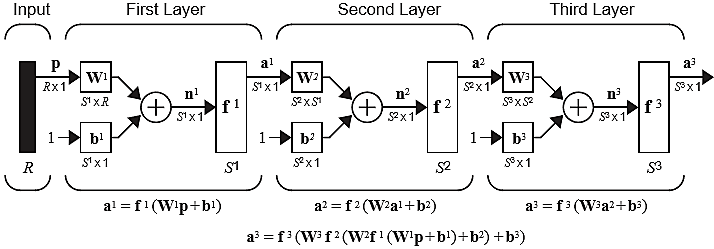
\includegraphics[width=16cm]{img/MLP.png}
        \caption{Perceptron de tres capas. \cite{libro1}}
        \label{fig:MLP}
    \end{center}
\end{figure}
Las principales aplicaciones del MLP son la clasificación de patrones y la aproximación de funciones. La aproximación de señales se usa en sistemas de control en donde se trata de encontrar una función que pueda mapear mediciones de salidas a controles de entrada. Se puede realizar la aproximación de cualquier función si se tienen suficientes neuronas en las capas ocultas. 
\subsection{Backpropagation}
Para el estudio de backpropagation es importante conocer las ecuaciones que se usan en el aprendizaje que realiza. La primera de ellas está relacionada con las salidas de cada capa del MLP, estas ecuaciones son otra forma de representar la arquitectura de la figura \ref{fig:MLP}.

\begin{equation} \label{eq:1}
\boldsymbol{a}^0 = \boldsymbol{p}
\end{equation}
\begin{equation} \label{eq:2}
\boldsymbol{a}^{m+1} = \boldsymbol{f}^{m+1}(\boldsymbol{W}^{m+1}\boldsymbol{a}^{m}+\boldsymbol{b}^{m+1}
), \text{Para $m=0, 1, \ldots M-1$}
\end{equation}
\begin{equation} \label{eq:3}
    \boldsymbol{a} = \boldsymbol{a}^{M}
\end{equation}
El valor de $M$ es el número de capas que tiene la red. La ecuación \ref{eq:1} hace referencia a que la capa uno tiene como entrada el conjunto de datos $\boldsymbol{p}$. Por otro lado la ecuación \ref{eq:3} es considerado como la salida final de la red neuronal.

El algoritmo backpropagation es una generalización del algoritmo LMS ya que ambos utilizan el error cuadrático medio, además utiliza un conjunto de entrenamiento compuesto por la entrada a la red y su correspondiente salida objetivo.
\[ \left\lbrace \boldsymbol{p_1}, \boldsymbol{t_1} \right\rbrace, \left\lbrace \boldsymbol{p_2}, \boldsymbol{t_2} \right\rbrace, \dots, \left\lbrace \boldsymbol{p_Q}, \boldsymbol{t_Q} \right\rbrace  \]

\subsection{ECUACIONES QUE PODRÍA ESTAR OCUPANDO}
\subsubsection{Forward propagation}
\begin{align*}
 \boldsymbol{a}^0 &= \boldsymbol{p} \\
 \boldsymbol{a}^{m+1} = 
\boldsymbol{f}^{m+1}(\boldsymbol{W}^{m+1}\boldsymbol{a}^{a}+\boldsymbol{b}^{m+1}
) & & \text{Para $m=0, 1, \ldots M-1$} \\
 \boldsymbol{a} &= \boldsymbol{a}^{M}
\end{align*}
\subsubsection{Backward propagation}
\begin{align*}
    \boldsymbol{s}^M &= 
-2\boldsymbol{\dot{F}}^{M}(\boldsymbol{n}^{M})(\boldsymbol{t-a}) \\
    \boldsymbol{s}^{m} &= 
\boldsymbol{\dot{F}}^{m}(\boldsymbol{n}^{m})(\boldsymbol{W}^{m+1})^{T}
\boldsymbol{s}^{m+1} & & \text{para $m=M-1, \ldots, 2, 1$} \\
\text{donde} \\
\boldsymbol{\dot{F}}^{m}(\boldsymbol{n}^{m}) &=
\begin{bmatrix}
  \dot{f}^{m}(n_{1}^{m}) & 0 & \ldots & 0 \\
  0 & \dot{f}^{m}(n_{2}^{m}) & \ldots & 0 \\
  \vdots & \vdots & \ddots & \vdots \\
  0 & 0 & \ldots & \dot{f}^{m}(n_{s^{m}}^{m})
\end{bmatrix} \\
\dot{f}^{m}(n_{j}^{m}) &= 
\frac{\partial \dot{f}^{m}(n_{j}^{m})}{\partial n_{j}^{m}}
\end{align*}
\subsubsection{Actualización de los pesos}
\begin{align*}
    \boldsymbol{W}^{m}(k+1) &= W^{m}(k)-\alpha 
\boldsymbol{s}^{m}(\boldsymbol{a}^{m-1})^{T}, \\
\boldsymbol{b}^{m}(k+1) &= \boldsymbol{b}^{m}(k) - \alpha \boldsymbol{s}^{m}
\end{align*}

\section{Resultados experimentales}
\subsection{Experimento 1}
\subsection{Experimento 2}
\subsection{Experimento 3}
\section{Discusión de resultados}
\section{Conclusiones}
\bibliographystyle{apalike}
\bibliography{reporte}
\section{Anexo}

\end{document}
